% Created 2020-10-29 Thu 14:53
% Intended LaTeX compiler: pdflatex
\documentclass[presentation]{beamer}
\usepackage[T1]{fontenc}
\setbeamerfont{frametitle}{size=\large}
\setbeamertemplate{footline}{
\begin{flushright}
\insertframenumber/\inserttotalframenumber\hspace{2mm}\mbox{}
\end{flushright}}
\usepackage[T1]{fontenc}
\usepackage{libertine}
\renewcommand*\familydefault{\sfdefault}
\usepackage[small]{eulervm}
\usepackage{tipa}
\usepackage{adjustbox}
\usepackage{multirow}
\usepackage{multicol}
\usepackage{tikz}
\usetikzlibrary{positioning}
\usepackage{tikz-qtree}
\usepackage{expex}
\usepackage{natbib}
\usepackage{stmaryrd}
\usepackage{stackrel}
\usepackage{stackengine}
\usepackage{relsize}
\usepackage{amsmath}
\usepackage{mathtools}
\usepackage{fixltx2e}
\usepackage{graphicx}
\usepackage{xcolor}
\usepackage[normalem]{ulem}
\bibliographystyle{li}
\usetheme{Boadilla}
\author{Julian Grove}
\date{October 28, 2020}
\title{Algebraic effects in Montague semantics}
\definecolor{gbbg}{HTML}{282828}
\definecolor{gbred}{HTML}{9d0006}
\definecolor{gblightred}{HTML}{cc241d}
\definecolor{gbgreen}{HTML}{79740e}
\definecolor{gbyellow}{HTML}{b57614}
\definecolor{gbblue}{HTML}{076678}
\definecolor{gbpurple}{HTML}{8f3f71}
\definecolor{gbaqua}{HTML}{427b58}
\definecolor{gbgray}{HTML}{928374}
\setbeamercolor*{structure}{fg=gbblue!70}
\setbeamercolor*{palette primary}{fg=white,bg=gbred!40}
\setbeamercolor*{palette secondary}{fg=white,bg=gbred!65}
\setbeamercolor*{palette tertiary}{fg=white,bg=gbred!90}
\setbeamercolor{section in toc}{fg=gbbg,bg=white}
\setbeamercolor{alerted text}{fg=gblightred}
\setbeamercolor{frametitle}{bg=gbgray!10!white,fg=gbblue}
\setbeamercolor{title}{fg=gbred}
\usepackage[linguistics]{forest}
\forestset{ downroof/.style={ for children={ if n=1{ edge path'={ (.parent first) -- (!u.parent anchor) -- (!ul.parent last) -- cycle }}{no edge} } } }
\newcommand{\lda}[2]{\lambda#1.#2}
\newcommand{\ctypeL}[2]{(#1\rightarrow#2)}
\newcommand{\ctypeR}[2]{#1\rightarrow#2}
\newcommand{\IF}[1]{\llbracket#1\rrbracket}
\newcommand{\app}[2]{#1(#2)}
\newlength\appwidth
\newcommand{\appS}[2]{\settowidth{\appwidth}{\ }#1\hspace{0.1\appwidth}#2}
\newcommand{\appC}[2]{\settowidth{\appwidth}{\ }(#1\hspace{0.1\appwidth}#2)}
\newcommand{\quant}[3]{#1#2:#3}
\newcommand{\ct}[1]{\textbf{#1}}
\newcommand{\stacks}[1]{\begin{tabular}{c}#1\end{tabular}}
\newcommand{\maybe}[1]{#1\textsubscript{$\#$}}
\def\divd{\ |\ }
\newcommand{\corners}[1]{\ulcorner#1\urcorner}
\newcommand{\uparrowed}[1]{\stackon[0pt]{$#1$}{$\uparrow$}}
\newcommand{\unit}[1]{#1^\eta}
\newlength\bindwidth
\newcommand{\bind}{\settowidth{\bindwidth}{\ }\mathtt{>\hspace{-1.7\bindwidth}>\hspace{-1.7\bindwidth}=}}
\newcommand{\abbrev}[1]{{\footnotesize\texttt{#1}}}
\def\ra{\rightarrow}
\newcommand{\dr}[1]{#1^\blacktriangleright}
\newlength\appendwidth
\newcommand{\append}[2]{\settowidth{\appendwidth}{\ }#1\hspace{-\appendwidth}::\hspace{-\appendwidth}#2}
\setbeamertemplate{frametitle continuation}{}
\institute[CLASP, U. of Gothenburg]{CLASP, University of Gothenburg}
\hypersetup{
 pdfauthor={Julian Grove},
 pdftitle={Algebraic effects in Montague semantics},
 pdfkeywords={},
 pdfsubject={},
 pdfcreator={Emacs 27.1 (Org mode 9.4)}, 
 pdflang={English}}
\begin{document}

\maketitle
\begin{frame}{Outline}
\tableofcontents
\end{frame}


\section{Side effects in linguistic semantics}
\label{sec:org04eba1d}

\begin{frame}[label={sec:org9f354ec}]{We are here}
\tableofcontents[currentsection]
\end{frame}

\begin{frame}[label={sec:org8cb4b8f}]{Semantics}
Semantics is for\ldots
\pause
\begin{itemize}[<+->]
\item characterizing semantic knowledge\ldots
\begin{itemize}
\item \ldots i.e., knowledge of \emph{entailments}? \emph{distributional properties}?
\end{itemize}
\item describing how linguistic structure (i.e., syntax) gives rise to the things being characterized (whatever they are)
\item describing how pragmatic stuff (e.g., presupposing something, referring to something, expressing something) should affect the things being characterized
\end{itemize}
\end{frame}

\begin{frame}[label={sec:org3f65adc}]{Montague}
\begin{center}
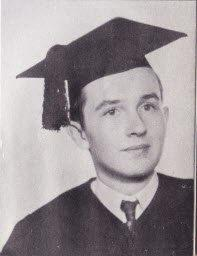
\includegraphics[width=60px]{./montague.jpg}
\end{center}
\pause
\begin{itemize}[<+->]
\item used models as a vehicle to characterize meanings in terms of entailments
\item described how linguistic structure gives rise to meanings, \emph{compositionally}
\begin{itemize}
\item simply typed \(\lambda\)-calculus
\end{itemize}
\item \alert{no} pragmatic stuff
\end{itemize}
\end{frame}

\begin{frame}[label={sec:org56ff3dc}]{Functional application}
\citealt{montague_proper_1973}:
\begin{center}
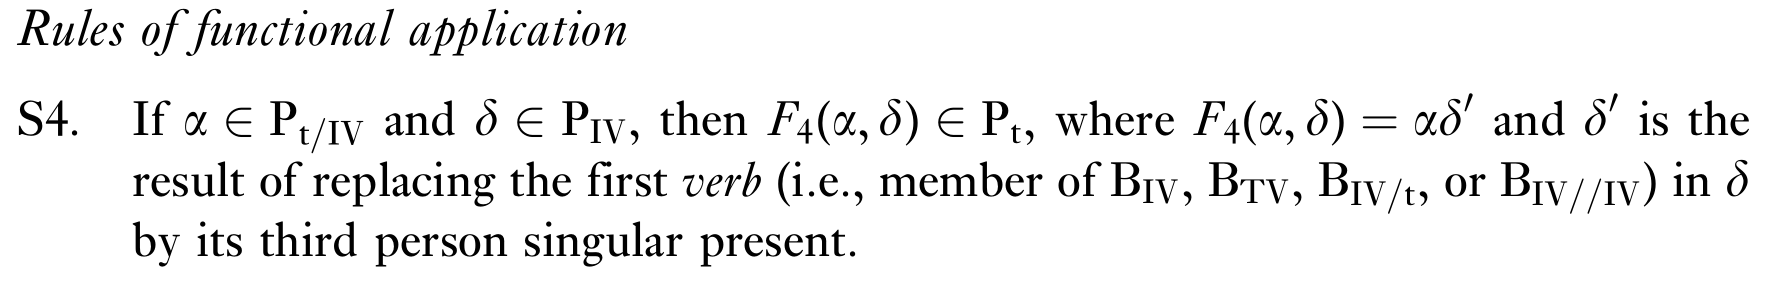
\includegraphics[width=300px]{./fa_syntax.jpg}
\end{center}
\begin{center}
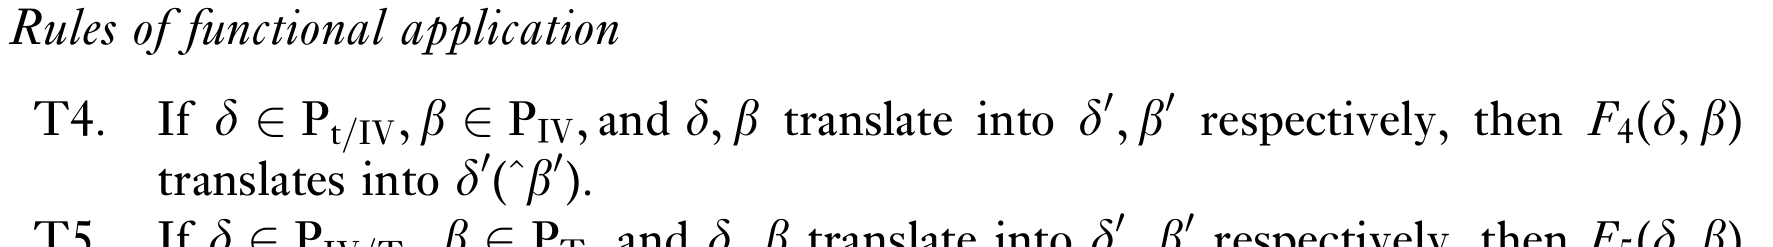
\includegraphics[width=300px]{./fa_semantics.jpg}
\end{center}

\centering
\begin{forest}
[[John][slept]]
\end{forest}
\begin{forest}
[\mbox{}\\$\leadsto$]
\end{forest}
\begin{forest}
[$\lda{s}{\appS{\appS{\ct{sleep}}{\ct{j}}}{s}}$ [$\lda{P, s}{\appS{\appS{P}{s}}{(\lda{s}{\ct{j}})}}$] [$\lda{s, x}{\appS{\appS{\ct{sleep}}{\appC{x}{s}}}{s}}$]]
\end{forest}
\end{frame}

\begin{frame}[label={sec:org0813fb0}]{Quantifying in}
\begin{center}
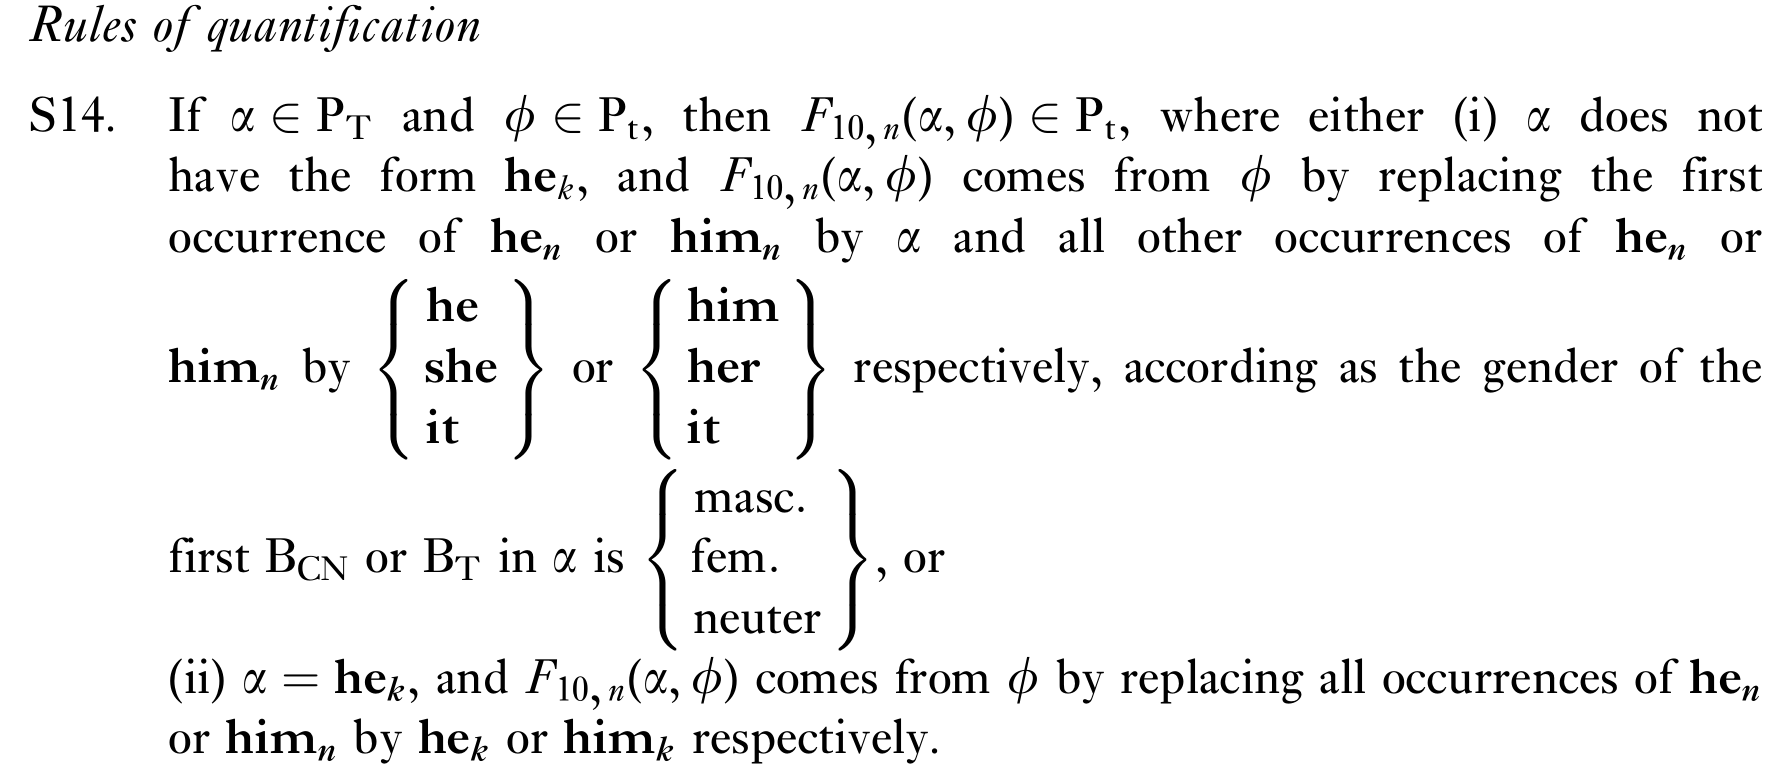
\includegraphics[width=300px]{./roq_syntax.jpg}
\end{center}
\begin{center}
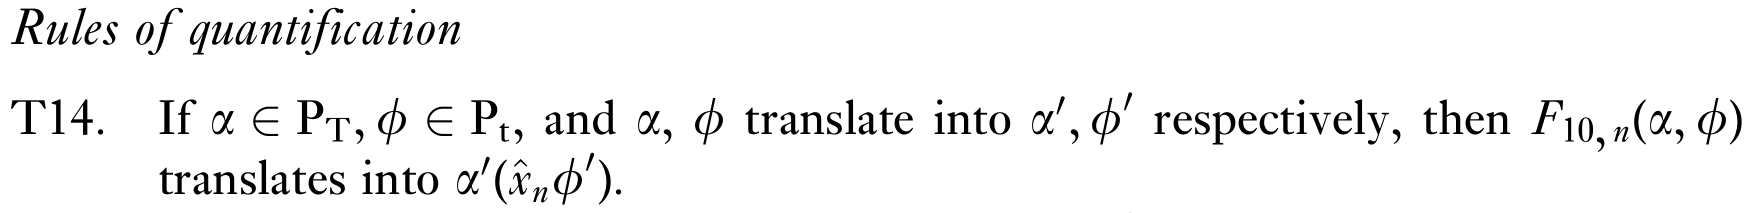
\includegraphics[width=300px]{./roq_semantics.jpg}
\end{center}
\end{frame}

\begin{frame}[label={sec:org26b117b}]{Quantifying in}
\emph{Every dog slept}\\
\centering
\begin{forest}
[[every dog] [he$_n$ slept]]
\end{forest}
\begin{forest}
[\mbox{}\\$\leadsto$]
\end{forest}{\small
\begin{forest}
[$\lda{s}{\quant{\forall}{u}{\appS{\appS{\ct{dog}}{u}}{s} \ra \appS{\appS{\ct{sleep}}{\underline{u}}}{s}}}$ [$\lda{P,s}{\quant{\forall}{u}{\appS{\appS{\ct{dog}}{u}}{s}} \ra \appS{\appS{P}{(\lda{s}{u})}}{s}}$] [$\lda{s}{\appS{\appS{\ct{sleep}}{\appC{\underline{x_n}}{s}}}{s}}$]]
\end{forest}}

\pause
\begin{center}
\alert{Not compositional}
\end{center}
\end{frame}

\begin{frame}[label={sec:orge13f6f1}]{Since then}
Many techniques since Montague for establishing seemingly non-local quantifier-variable dependencies\ldots
\pause
\begin{itemize}[<+->]
\item Cooper Storage and variants thereof \citep{cooper_quantification_1983,keller_nested_1988}
\item Quantifier Raising and Predicate Abstraction \citep{heim_semantics_1998}
\item Flexible types and/or combinators \citep{hendriks_studied_1993,steedman_syntactic_2000}
\item Grammars with interfaces to side effects
\begin{itemize}
\item Continuations \citep{barker_continuations_2002,barker_continuations_2014}
\item Monads \citep{shan_monads_2002,charlow_semantics_2014}
\item Idioms \citep{kobele_cooper_2018}
\end{itemize}
\end{itemize}
\end{frame}

\begin{frame}[label={sec:orga6e8859}]{Side effects}
Programming languages may exhibit "impure" behaviors.
\pause
\begin{itemize}[<+->]
\item input/output
\begin{itemize}
\item print "hi"
\end{itemize}
\item environment/state
\begin{itemize}
\item os.path.exists("./gremlins2.mov")
\end{itemize}
\item partiality/exceptions
\item non-determinism
\end{itemize}

\pause
\emph{Pure} programs merely manipulate data\ldots
\pause
\begin{itemize}
\item e.g., through functional application
\begin{itemize}
\item def add(x, y):\\
\hspace{5mm}return (x + y)
\end{itemize}
\end{itemize}

\bigskip

\pause
\alert{Theories of side effects (e.g., monads) provide interfaces to impure behavior.} 
\end{frame}

\begin{frame}[label={sec:org1b64c63}]{Linguistic side effects}
The effectful approach:
\pause
\begin{itemize}[<+->]
\item identity linguistic phenomenon that appears to behave ``impurely'', i.e., by subverting compositionality
\begin{itemize}
\item e.g., quantification, anaphora, conventional implicature\ldots
\end{itemize}
\item find an effectful interface that appropriately describes its behavior
\item add it to your compositional repertoire!
\end{itemize}
\end{frame}

\begin{frame}[label={sec:org74cfb39}]{This talk}
\begin{itemize}[<+->]
\item present two monadic interfaces to side effects: one for quantification and one anaphora
\begin{itemize}
\item the Continuation monad and the State monad, respectively
\item analyses inspired by \cite{charlow_semantics_2014}
\end{itemize}
\item show how they may and \emph{may not} be combined
\item introduce \emph{algebraic effects}
\end{itemize}
\end{frame}

\begin{frame}[label={sec:orgb213b97}]{Monads}
a functor \(\mathcal{M}\), equipped with two operators, \(\unit{(\cdot)}\) (`return') and \(\bind\) (`bind')

\bigskip

\begin{columns}
\begin{column}{0.5\columnwidth}
\begin{definition}[\(\mathcal{M}\)]
\vspace{-5mm}
\begin{align*}
\mathcal{M} &: \mathcal{T} \ra \mathcal{T}\\
\unit{(\cdot)} &: a \ra \mathcal{M}(a)\\
(\bind) &: \mathcal{M}(a) \ra (a \ra \mathcal{M}(b)) \ra \mathcal{M}(b)
\end{align*}
\end{definition}
\end{column}
\end{columns}

\bigskip \pause

Intuitively: \(\mathcal{M}(a)\) is the space where the side effects of some value of type \(a\) happen.
\pause
\begin{itemize}[<+->]
\item \(\unit{(\cdot)}\) lifts pure values into that space.
\item \(\bind\) sequences programs inhabiting that space by binding the result of one to the input of the next.
\end{itemize}

\pause
\begin{center}
\alert{The operators must satisfy the Monad Laws.}
\end{center}
\end{frame}

\begin{frame}[label={sec:org0274f58}]{The Monad Laws}
\begin{align*}
\unit{v}\ \bind\ k &= k v\tag{Left Identity}\\[2mm]
m\ \bind\ \lda{v}{\unit{v}} &= m\tag{Right Identity}\\[2mm]
(m\ \bind\ n)\ \bind\ o &= m\ \bind\ \lda{v}{\appS{n}{v}\ \bind\ o}\tag{Associativity}
\end{align*}
\end{frame}

\begin{frame}[label={sec:org2709847}]{First case: quantification}
In the Continuation monad, scope-taking is a kind of side effect.

\begin{columns}
\begin{column}{0.5\columnwidth}
\begin{definition}[\(\mathcal{C}\)]
\vspace{-5mm}
\begin{align*}
\onslide<1->{\mathcal{C}(a) :\ &(a \ra o) \ra o\\[3mm]}
\onslide<2->{\unit{(\cdot)} :\ &a \ra (a \ra o) \ra o\\}
\onslide<3->{\unit{v} =\ &\lda{c}{\appS{c}{v}}\\[3mm]}
\onslide<4->{(\bind) :\ &((a \ra o) \ra o)\\
\ra\ &(a \ra (b \ra o) \ra o)\\
\ra\ &(b \ra o) \ra o\\}
\onslide<5>{m\ \bind\ k =\ &\lda{c}{m (\lda{v}{\appS{\appS{k}{v}}{c}})}}
\end{align*}
\end{definition}
\end{column}
\end{columns}
\end{frame}

\begin{frame}[label={sec:org508c9a3},t]{How it works}
\begin{enumerate}
\item Ashley hugged every dog.
\end{enumerate}

\only<2>{
\begin{align*}
\abbrev{ashley} &= \unit{\ct{a}} : \mathcal{C}(e)\tag{Lexicon}\\
\abbrev{hugged} &= \unit{\ct{hug}} : \mathcal{C}(e \ra t)\\
\abbrev{every} &= \lda{P, c}{\quant{\forall}{x}{\appS{P}{x} \ra \appS{c}{x}}} : (e \ra t) \ra (e \ra t) \ra t\\
\abbrev{dog} &= \ct{dog} : e \ra t
\end{align*}
\only<4>{\begin{align*}
(\triangleright) &: \mathcal{C}(a \ra b) \ra \mathcal{C}(a) \ra \mathcal{C}(b)\tag{Grammar}\\
m \triangleright n &= m\ \bind\ \lda{f}{n\ \bind\ \lda{x}{\unit{\appC{f}{x}}}}\\
&= \lda{c}{\appS{m}{(\lda{f}{\appS{n}{(\lda{x}{\appS{c}{\appC{f}{x}}})}})}}\\[2mm]
(\triangleleft) &: \mathcal{C}(a) \ra \mathcal{C}(a \ra b) \ra \mathcal{C}(b)\\
m \triangleleft n &= m\ \bind\ \lda{x}{n\ \bind\ \lda{f}{\unit{\appC{f}{x}}}}\\
&= \lda{c}{\appS{m}{(\lda{x}{\appS{n}{(\lda{f}{\appS{c}{\appC{f}{x}}})}})}}
\end{align*}}
}
\only<3-4>{
\begin{align*}
\abbrev{ashley} &= \unit{\ct{a}} : \mathcal{C}(e)\tag{Lexicon}\\
\abbrev{hugged} &= \unit{\ct{hug}} : \mathcal{C}(e \ra t)\\
\abbrev{every} &= \lda{P, c}{\quant{\forall}{x}{\appS{P}{x} \ra \appS{c}{x}}} : (e \ra t) \ra \mathcal{C}(e)\\
\abbrev{dog} &= \ct{dog} : e \ra t
\end{align*}
\only<4>{\begin{align*}
(\triangleright) &: \mathcal{C}(a \ra b) \ra \mathcal{C}(a) \ra \mathcal{C}(b)\tag{Grammar}\\
m \triangleright n &= m\ \bind\ \lda{f}{n\ \bind\ \lda{x}{\unit{\appC{f}{x}}}}\\
&= \lda{c}{\appS{m}{(\lda{f}{\appS{n}{(\lda{x}{\appS{c}{\appC{f}{x}}})}})}}\\[2mm]
(\triangleleft) &: \mathcal{C}(a) \ra \mathcal{C}(a \ra b) \ra \mathcal{C}(b)\\
m \triangleleft n &= m\ \bind\ \lda{x}{n\ \bind\ \lda{f}{\unit{\appC{f}{x}}}}\\
&= \lda{c}{\appS{m}{(\lda{x}{\appS{n}{(\lda{f}{\appS{c}{\appC{f}{x}}})}})}}
\end{align*}}
}
\centering
\only<5->{\bigskip\bigskip\bigskip\bigskip}
\only<5>{$\abbrev{ashley} \triangleleft (\abbrev{hugged} \triangleright \appS{\abbrev{every}}{\abbrev{dog}})$}
\only<6-7>{$\unit{\ct{a}} \triangleleft (\unit{\ct{hug}} \triangleright \appS{\abbrev{every}}{\ct{dog}})$\\\bigskip\bigskip\only<7>{expand $\appS{\abbrev{every}}{\ct{dog}}$\ldots}}
\only<8-9>{$\unit{\ct{a}} \triangleleft (\unit{\ct{hug}} \triangleright \lda{c}{\quant{\forall}{x}{\appS{\ct{dog}}{x} \ra \appS{c}{x}}})$\\\bigskip\bigskip\only<9>{expand $\triangleright$\ldots}}
\only<10-11>{$\unit{\ct{a}} \triangleleft \lda{c}{\quant{\forall}{x}{\appS{\ct{dog}}{x} \ra \appS{c}{\appC{\ct{hug}}{x}}}}$\\\bigskip\bigskip\only<11>{expand $\triangleleft$\ldots}}
\only<12-13>{$\lda{c}{\quant{\forall}{x}{\appS{\ct{dog}}{x} \ra \appS{c}{\appC{\appS{\ct{hug}}{x}}{\ct{a}}}}}$\\\bigskip\bigskip\only<13>{to obtain a proposition, apply to the identity function\ldots}}
\only<14>{$\quant{\forall}{x}{\appS{\ct{dog}}{x} \ra \appS{\appS{\ct{hug}}{x}}{\ct{a}}}$}
\end{frame}

\begin{frame}[label={sec:org798a1ee}]{Summary}
Using continuations to manage scope-taking:
\pause
\begin{itemize}[<+->]
\item scopal expressions take scope over their continuations, which are reified as they compose
\item values take scope trivially (applying Montague's ``lift'')
\end{itemize}
\end{frame}

\begin{frame}[label={sec:orgd19f5a3}]{Second case: anaphora}
In the State monad, we may read from and write to an environment.
\begin{columns}
\begin{column}{0.5\columnwidth}
\begin{definition}[\(\mathcal{S}\)]
\vspace{-5mm}
\begin{align*}
\onslide<1->{\mathcal{S}(a) :\ &s \ra (s, a)\\[3mm]}
\onslide<2->{\unit{(\cdot)} :\ &a \ra s \ra (s, a)\\}
\onslide<3->{\unit{v} =\ &\lda{s}{\langle s, v\rangle}\\[3mm]}
\onslide<4->{(\bind) :\ &(s \ra (s, a))\\
\ra\ &(a \ra s \ra (s, b))\\
\ra\ &s \ra (s, b)\\}
\onslide<5>{m\ \bind\ k =\ &\lda{s}{\abbrev{let}\ \langle s^\prime, v\rangle = m s\ \abbrev{in}\ \appS{\appS{k}{v}}{s^\prime}}}
\end{align*}
\end{definition}
\end{column}
\end{columns}
\end{frame}

\begin{frame}[label={sec:org2fc1175},t]{How it works}
\begin{enumerate}
\item Ashley hugged herself.
\end{enumerate}

\only<2>{
\begin{align*}
\abbrev{ashley} &= \unit{\ct{a}} : \mathcal{S}(e)\tag{Lexicon}\\
\abbrev{hugged} &= \unit{\ct{hug}} : \mathcal{S}(e \ra t)\\
\abbrev{herself} &= \lda{s}{\langle s, \appS{\abbrev{sel}}{s}\rangle} : s \ra (s, e)
\end{align*}}
\only<3>{\begin{align*}
\abbrev{ashley} &= \unit{\ct{a}} : \mathcal{S}(e)\tag{Lexicon}\\
\abbrev{hugged} &= \unit{\ct{hug}} : \mathcal{S}(e \ra t)\\
\abbrev{herself} &= \lda{s}{\langle s, \appS{\abbrev{sel}}{s}\rangle} : \mathcal{S}(e)
\end{align*}}
\only<4-5>{\begin{align*}
(\triangleright) &: \mathcal{S}(a \ra b) \ra \mathcal{S}(a) \ra \mathcal{S}(b)\tag{Grammar}\\
m \triangleright n &= m\ \bind\ \lda{f}{n\ \bind\ \lda{x}{\unit{\appC{f}{x}}}}\\
&= \lda{s}{\abbrev{let}\ \langle f, s^\prime\rangle = \appS{m}{s}\ \abbrev{in}\ \abbrev{let}\ \langle x, s^{\prime\prime}\rangle = \appS{n}{s^\prime}\ \abbrev{in}\ \langle\appS{f}{x}, s^{\prime\prime}\rangle}\\[3mm]
(\triangleleft) &: \mathcal{S}(a) \ra \mathcal{S}(a \ra b) \ra \mathcal{S}(b)\\
m \triangleleft n &= m\ \bind\ \lda{x}{n\ \bind\ \lda{f}{\unit{\appC{f}{x}}}}\\
&= \lda{s}{\abbrev{let}\ \langle x, s^\prime\rangle = \appS{m}{s}\ \abbrev{in}\ \abbrev{let}\ \langle f, s^{\prime\prime}\rangle = \appS{n}{s^\prime}\ \abbrev{in}\ \langle\appS{f}{x}, s^{\prime\prime}\rangle}\\[4mm]
\onslide<5>{\dr{(\cdot)} &: \mathcal{S}(e) \ra \mathcal{S}(e)\\
\dr{m} &= m\ \bind\ \lda{x, s}{\langle\append{x}{s}, x\rangle}}
\end{align*}}
\centering
\only<6->{\bigskip\bigskip\bigskip\bigskip}
\only<6>{$\dr{\abbrev{ashley}} \triangleleft (\abbrev{hugged} \triangleright \abbrev{herself})$}
\only<7>{$\dr{\abbrev{ashley}} \triangleleft (\unit{\ct{hug}} \triangleright \abbrev{herself})$}
\only<8>{$(\lda{s}{\langle\append{\ct{a}}{s}, \ct{a}\rangle)} \triangleleft (\unit{\ct{hug}} \triangleright \abbrev{herself})$}
\only<9-10>{$(\lda{s}{\langle\append{\ct{a}}{s}, \ct{a}\rangle)} \triangleleft (\unit{\ct{hug}} \triangleright \lda{s}{\langle s,\appS{\abbrev{sel}}{s}\rangle})$\\\bigskip\bigskip\only<10>{expand $\triangleright$\ldots}}
\only<11-12>{$(\lda{s}{\langle\append{\ct{a}}{s}, \ct{a}\rangle)} \triangleleft \lda{s}{\langle s,\appS{\ct{hug}}{\appC{\abbrev{sel}}{s}}\rangle}$\\\bigskip\bigskip\only<12>{expand $\triangleleft$\ldots}}
\only<13>{$\lda{s}{\langle\append{\ct{a}}{s}, \appS{\appS{\ct{hug}}{\appC{\abbrev{sel}}{(\append{\ct{a}}{s})}}}{\ct{a}}\rangle}$}
\end{frame}

\begin{frame}[label={sec:org28aaae9}]{Summary}
Using State to manage anaphora:
\pause
\begin{itemize}[<+->]
\item expressions that introduce discourse referents or engage in anaphora engage with the environment
\item values are trivially stateful, by passing the environment on, untouched
\end{itemize}
\end{frame}

\begin{frame}[label={sec:orgbc5890c}]{Combining quantification and anaphora}
How might one do this?\\

\bigskip \pause

Answer: one may use \emph{monad transformers} (the strategy adopted by \cite{shan_monads_2002}, and then, by \cite{charlow_semantics_2014}).
\end{frame}

\begin{frame}[label={sec:orgddc2b6f}]{Monad transformers}
\(\mathcal{C}\) and \(\mathcal{S}\) are associated with corresponding monad transformers, \(\mathcal{C}_T\) and \(\mathcal{S}_T\).

\begin{columns}
\begin{column}{0.8\columnwidth}
\begin{definition}[\(\mathcal{M}_T\)]
\vspace{-5mm}
\begin{align*}
\mathcal{M}_T &: (\mathcal{T} \ra \mathcal{T}) \ra \mathcal{T} \ra \mathcal{T}\\
\unit{(\cdot)} &: a \ra \mathcal{M}_T(\mathcal{M}_0)(b)\\
(\bind) &: \mathcal{M}_T(\mathcal{M}_0)(a) \ra (a \ra \mathcal{M}_T(\mathcal{M}_0)(b)) \ra \mathcal{M}_T(\mathcal{M}_0)(b)
\end{align*}
\end{definition}
\end{column}
\end{columns}

\bigskip
given one of \(\mathcal{C}\) or \(\mathcal{S}\) as the \emph{underlying monad}, we may apply one of \(\mathcal{S}_T\) or \(\mathcal{C}_T\) to it\ldots
\end{frame}

\begin{frame}[label={sec:org7431951}]{The Continuation monad transformer}
\begin{columns}
\begin{column}{0.75\columnwidth}
\begin{definition}[\(\mathcal{C}_T\)]
\vspace{-5mm}
\begin{align*}
\mathcal{C}_T(\mathcal{M}_0)(a) :\ &(a \ra \mathcal{M}_0(o)) \ra \mathcal{M}_0(o)\\[3mm]
\unit{(\cdot)} :\ &a \ra (a \ra \mathcal{M}_0(o)) \ra \mathcal{M}_0(o)\\
\unit{v} =\ &\lda{c}{\appS{c}{v}}\\[3mm]
(\bind) :\ &((a \ra \mathcal{M}_0(o)) \ra \mathcal{M}_0(o))\\
\ra\ &(a \ra (b \ra \mathcal{M}_0(o)) \ra \mathcal{M}_0(o))\\
\ra\ &(b \ra \mathcal{M}_0(o)) \ra \mathcal{M}_0(o)\\
m\ \bind\ k =\ &\lda{c}{m (\lda{v}{\appS{\appS{k}{v}}{c}})}
\end{align*}
\end{definition}
\end{column}
\end{columns}
\end{frame}

\begin{frame}[label={sec:org5561de4}]{The State monad transformer}
\begin{columns}
\begin{column}{0.75\columnwidth}
\begin{definition}[\(\mathcal{S}_T\)]
\vspace{-5mm}
\begin{align*}
\mathcal{S}_T(\mathcal{M}_0)(a) :\ &s \ra \mathcal{M}_0((s, a))\\[3mm]
\unit{(\cdot)} :\ &a \ra s \ra \mathcal{M}_0((s, a))\\
\unit{v} =\ &\lda{s}{\unit{\langle s, v\rangle}}\\[3mm]
(\bind) :\ &(s \ra \mathcal{M}_0((s, a)))\\
\ra\ &(a \ra (s \ra \mathcal{M}_0((s, b))))\\
\ra\ &s \ra \mathcal{M}_0((s, b))\\
m\ \bind\ k =\ &\lda{s}{\appS{m}{s}\ \bind\ \lda{p}{\abbrev{let}\ \langle s^\prime, v\rangle = p\ \abbrev{in}\ \appS{\appS{k}{v}}{s^\prime}}}
\end{align*}
\end{definition}
\end{column}
\end{columns}
\end{frame}

\begin{frame}[label={sec:org63fa88c}]{To summarize\ldots}
This general strategy can be made to work extremely well \citep{charlow_semantics_2014}.

\bigskip \pause
But, how do we decide which monad transformer to apply to which monad?  
\pause
\begin{enumerate}
\item Every dog licked Ashley. *It is friendly.
\end{enumerate}

\bigskip \pause
It turns out we must apply \(\mathcal{C}_T\) to \(\mathcal{S}\) and \alert{not} \(\mathcal{S}_T\) to \(\mathcal{C}\).

\bigskip \pause
If we adopt the transformers approach from the start\ldots
\pause
\begin{itemize}[<+->]
\item we throw out our generalized quantifier meaning for \emph{every dog}
\item the type of \emph{every dog} becomes \((e \ra \mathcal{M}_0(t)) \ra \mathcal{M}_0(t)\) \ldots
\begin{itemize}
\item but a generic meaning for \emph{every} cannot be written\ldots we are required to know what \(\mathcal{M}_0\) is!
\item even then, the meaning the quantifier will be somewhat stipulative, e.g., to account for the data above (though, it can be made to follow from a small set of primitives, as in \cite{charlow_semantics_2014})
\end{itemize}
\end{itemize}
\end{frame}

\begin{frame}[label={sec:org9af8e2f}]{The problem}
The transformers approach, when used generically, prevents us from writing meanings. When used non-generically, it loses extensibility.

\bigskip \pause
Might we salvage our individual analyses in some other way? In doing so, might we account for data like (1)?
\end{frame}

\section{Algebraic effects and handlers}
\label{sec:org5832ec0}

\begin{frame}[label={sec:org2e05c38}]{We are here}
\tableofcontents[currentsection]
\end{frame}

\begin{frame}[label={sec:org527ec96}]{Background}
Algebraic effects and handlers provide a means of writing extensible code, recently especially popular in functional programming.\footnote{Original insights about the relation between algebra and computational effects are from \citealt{plotkin_semantics_2001,plotkin_algebraic_2003}.} 

\bigskip \pause
Jirka Mar\v{s}{\'i}k has done significant work importing algebraic effects into linguistic semantics, culminating in his dissertation \citep{marsik_algebraic_2014,marsik_introducing_2016,marsik_effects_2016}
\pause
\begin{itemize}[<+->]
\item develops a typed extension of \(\lambda\)-calculus
\item studies an array of phenomena algebraically, including quantification, presupposition, conventional implicature, and deixis
\item anaphora is approached using the compositional DRT of \cite{degroote_towards_2006}
\end{itemize}
\end{frame}

\begin{frame}[label={sec:orgea28ebe}]{The basic idea}
Instead of fixing a monad transformer stack, we may study the side effects of individual phenomena independently\ldots
\pause
\begin{itemize}[<+->]
\item by characterizing them algebraically
\item and then combining the resulting algebras
\end{itemize}

\bigskip \pause
I will take a different approach from Mar\v{s}{\'i}k, by\ldots
\pause
\begin{itemize}[<+->]
\item staying in STLC (with unit)
\item characterizing anaphora in purely algebraic terms
\item sticking with a traditional analysis of quantifiers, i.e., whereon they denote sets of sets
\end{itemize}
\end{frame}

\begin{frame}[label={sec:orgc5f668c}]{Algebraic signatures}
An algebraic signature is a set \(E\) of operations, each one associated with a \emph{parameter} \(p\) and an \emph{arity} \(a\) (both types), along with a special operation \(\eta\) (`return').

\begin{center}
\(E = \{{\abbrev{op}_1}_{p_1 \leadsto a_1}, \ldots, {\abbrev{op}_n}_{p_n \leadsto a_n}, \eta\}\)
\end{center}

\pause
Elements of the algebra with signature \(E\) inhabit a type which we call \(\mathcal{F}_E(v)\) (for some \emph{return} type \(v\)).

\bigskip \pause
To say operator \(\abbrev{op}_{p \leadsto a}\) is in signature \(E\) means that it has the following type signature:
\begin{center}
\(\abbrev{op}_{p \leadsto a} : p \ra (a \ra \mathcal{F}_{E}(v)) \ra \mathcal{F}_E(v)\)
\end{center}

\bigskip \pause
\(\eta\) always has the following type signature:
\begin{center}
\(\eta : v \ra \mathcal{F}_E(v)\)
\end{center}
\end{frame}

\begin{frame}[label={sec:orged14d7b}]{Algebraic laws}
In addition to the signature, an algebra determines a set of equations that must hold among its elements, of the form
\begin{center}
\(\abbrev{op}_i(p_i; \ldots) = \abbrev{op}_j(p_j; \ldots)\)
\end{center}
\end{frame}

\begin{frame}[label={sec:org3c01693}]{The State algebra (signature)}
instead of a State monad, we will have a State algebra

\bigskip \pause
two operations, \(\abbrev{get}_{\star \leadsto s}\) and \(\abbrev{put}_{s \leadsto \star}\)
\pause
\begin{itemize}[<+->]
\item \(s\) is the type of the state
\item \(\star\) is the unit type (one inhabitant, also called \(\star\))
\end{itemize}

\bigskip \pause
Some example elements of the State algebra\ldots
\pause
\begin{itemize}[<+->]
\item \(\abbrev{get}_{\star \leadsto s}(\star; \lda{s}{\appS{\eta}{s}}) : \mathcal{F}_{\{\abbrev{get}_{\star \leadsto s}, \abbrev{put}_{s \leadsto \star}\}}(s)\)
\item \(\abbrev{get}_{\star \leadsto s}(\star; \lda{s}{\abbrev{put}_{s \leadsto \star}(\append{\ct{a}}{s}; \lda{\star}{\appS{\eta}{s}})}) : \mathcal{F}_{\{\abbrev{get}_{\star \leadsto s}, \abbrev{put}_{s \leadsto \star}\}}(s)\)
\item \(\abbrev{get}_{\star \leadsto s}(\star; \lda{s}{\abbrev{put}_{s \leadsto \star}(\append{\ct{a}}{s}; \lda{\star}{\appS{\eta}{\ct{a}}})}) : \mathcal{F}_{\{\abbrev{get}_{\star \leadsto s}, \abbrev{put}_{s \leadsto \star}\}}(e)\)
\end{itemize}
\end{frame}

\begin{frame}[label={sec:org654df84}]{The State algebra (laws)}
Reading the environment twice is no better than reading it once:
\begin{center}
\(\abbrev{get}_{\star \leadsto s}(\star; \lda{g}{\abbrev{get}_{\star \leadsto s}(\star; \lda{g^\prime}{\appS{\appS{k}{g}}{g^\prime}})}) = \abbrev{get}_{\star \leadsto s}(\star; \lda{g}{\appS{\appS{k}{g}}{g}})\)
\end{center}

\bigskip \pause
Putting something back where you got it is the same as doing nothing:
\begin{center}
\(\abbrev{get}_{\star \leadsto s}(\star; \lda{g}{\abbrev{put}_{s \leadsto \star}(g; k)})) = k \star\)
\end{center}

\bigskip \pause
Getting after you just put means getting what you put:
\begin{center}
\(\abbrev{put}_{s \leadsto \star}(g; \lda{\star}{\abbrev{get}_{\star \leadsto s}(\star; k)}) = \abbrev{put}_{s \leadsto \star}(g; \lda{\star}{\appS{k}{g}})\)
\end{center}

\bigskip \pause
Putting twice overwrites:
\begin{center}
\(\abbrev{put}_{s \leadsto \star}(g; \lda{\star}{\abbrev{put}_{s \leadsto \star}(g^\prime; k)}) = \abbrev{put}_{s \leadsto \star}(g^\prime; k)\)
\end{center}
\end{frame}

\begin{frame}[label={sec:orgc89eea9}]{The Quantifier algebra (signature)}
one operation, \(\abbrev{scope}_{(e \ra t) \ra t \leadsto e}\)

\bigskip \pause
Some example elements of the Quantifier algebra\ldots
\begin{itemize}
\item \small \(\abbrev{scope}_{(e \ra t) \ra t \leadsto e}(\appS{\abbrev{every}}{\ct{dog}}; \lda{y}{\appS{\eta}{\appC{\ct{sleep}}{y}}}) : \mathcal{F}_{\{\abbrev{scope}_{(e \ra t) \ra t \leadsto e}\}(t)}\)
\item \footnotesize \(\abbrev{scope}_{(e \ra t) \ra t \leadsto e}(\appS{\abbrev{every}}{\ct{dog}}; \lda{y}{\abbrev{scope}_{(e \ra t) \ra t \leadsto e}(\appS{\abbrev{every}}{\ct{cat}}; \lda{z}{\appS{\eta}{\appC{\appS{\ct{chase}}{z}}{y}}})}) : \mathcal{F}_{\{\abbrev{scope}_{(e \ra t) \ra t \leadsto e}\}(t)}\)
\end{itemize}
\end{frame}

\begin{frame}[label={sec:org9ce1638}]{The Quantifier algebra (laws)}
Quantifying in:
\begin{center}
\(\abbrev{scope}_{(e \ra t) \ra t \leadsto e}(q; \lda{x}{\appS{\eta}{\appC{k}{x}}}) = \appS{\eta}{\appC{q}{k}}\)
\end{center}
\end{frame}

\begin{frame}[label={sec:org28f3d3a}]{Combing the algebras\ldots}
is just a matter of
\pause
\begin{itemize}[<+->]
\item collecting the operations into one signature
\item combining the equations
\item adding one more law to allow \(\abbrev{scope}_{(e \ra t) \ra t \leadsto e}\) to commute with \(\abbrev{get}_{\star \leadsto s}\) and \(\abbrev{put}_{s \leadsto \star}\)
\end{itemize}

\bigskip \pause
Commuting \(\abbrev{scope}_{(e \ra t) \ra e \leadsto e}\) past \(\abbrev{get}_{\star \leadsto s}\) and \(\abbrev{put}_{s \leadsto \star}\):
\begin{center}
\(\abbrev{scope}_{(e \ra t) \ra e \leadsto e}(q; \lda{x}{\abbrev{get}_{\star \leadsto s}(\star; \lda{s}{\abbrev{put}_{s \leadsto \star}(s^\prime; \lda{\star}{\appS{\appS{\appS{k}{x}}}{s}}{s^\prime})})})\)
\bigskip

= \(\abbrev{get}_{\star \leadsto s}(\star; \lda{s}{\abbrev{put}_{s \leadsto \star}(s; \lda{\star}{\abbrev{scope}_{(e \ra t) \ra e \leadsto e}(q; \lda{x}{\appS{\appS{\appS{k}{x}}{s}}{s^\prime}})})})\)
\end{center}
\end{frame}

\section{Making it Montagovian}
\label{sec:org155b505}

\begin{frame}[label={sec:org04751ea}]{We are here}
\tableofcontents[currentsection]
\end{frame}

\begin{frame}[label={sec:org372f31b}]{How to do it}
What we want is an encoding of the operations, as well as a way of \emph{translating} \(\lambda\)-terms with lots of operations into ones with fewer operations in a way that respects the algebraic laws.

\bigskip \pause
This is called ``handling'' the operations. It can treat algebraic laws essentially as \emph{reduction rules}. From this perspective, we may obtain a ``normal form'' for algebraic elements.

\bigskip \pause
In the combined State/Quantifier algebra, the normal form for any element is determined by the laws to be
\begin{center}
\(\abbrev{get}_{\star \leadsto s}(\star; \lda{s}{\abbrev{put}_{\star \leadsto s}(\appS{f}{s}; \appS{\eta}{\appC{g}{s}})})\)
\end{center}

for some \(f: s \rightarrow s\) and \(g: s \rightarrow v\).

\bigskip \pause
Pairs of such functions \(f\) and \(g\) can be represented as \(\lda{s}{\langle\appS{f}{s}, \appS{g}{s}\rangle}\) \ldots they are State monadic!
\end{frame}

\begin{frame}[label={sec:orgf4e7aa6}]{Encoding elements}
To encode elements of an algebra, we define a family of functors \(\mathcal{F} : \mathcal{T}_\leadsto^* \ra \mathcal{T} \ra \mathcal{T}\), where
\begin{itemize}
\item \(\mathcal{T}_\leadsto^*\) is the free monoid (i.e., of lists) over \(\mathcal{T}_\leadsto = \{p \leadsto a \divd p, a \in \mathcal{T}\}\)
\end{itemize}

\pause\vspace{-5mm}
\begin{align*}
\mathcal{F}_\epsilon(v) &= v\\
\mathcal{F}_{p \leadsto a, l}(v) &= (p \ra (a \ra \mathcal{F}_l(v)) \ra o) \ra o 
\end{align*}\vspace{-12mm}

\pause
\begin{align*}
\abbrev{op}_{p \leadsto a} &: p \ra (a \ra \mathcal{F}_l(v)) \ra \mathcal{F}_{p \leadsto a, l}\\
\abbrev{op}_{p \leadsto a}(p; k) &= \lda{h}{\appS{\appS{h}{p}}{k}}\\[2mm]
\onslide<4->{\eta &: v \ra \mathcal{F}_\epsilon(v)\\
\appS{\eta}{v} &= v}
\end{align*}

\pause \pause
Operations construct ``pairs''; returning just returns\ldots
\end{frame}

\begin{frame}[label={sec:org49cf6c3}]{An element of the State/Quantifier algebra}
\begin{enumerate}
\item Every dog hugged itself.
\end{enumerate}

\bigskip \pause
$\abbrev{scope}_{(e \ra t) \ra t \leadsto e}(\appS{\abbrev{every}}{\ct{dog}};$\\
$\hspace{1cm}\lda{x}{\abbrev{get}_{\star \leadsto s}(\star;$\\
$\hspace{2cm}\lda{s}{\abbrev{put}_{s \leadsto \star}(\append{x}{s};$\\
$\hspace{3cm}\lda{\star}{\abbrev{get}_{\star \leadsto s}(\star; \lda{s^\prime}{\appS{\eta}{\appC{\appS{\ct{hug}}{\appC{\abbrev{sel}}{s^\prime}}}{x}}})})})})$

\bigskip \pause
\begin{center}
\(= \lda{h}{\appS{\appS{h}{\appC{\abbrev{every}}{\ct{dog}}}}{(\lda{x, h^\prime}{\appS{\appS{h^\prime}{\star}}{(\lda{s}{\ldots})})}}}\)
\end{center}

\bigskip \pause
This will be an expression of type
\begin{align*}
&\mathcal{F}_{(e \ra t) \ra t \leadsto e, \star \leadsto s, s \leadsto \star, \star \leadsto s}\\
=\ \ &(((e \ra t) \ra t) \ra (e \ra ((\star \ra (s \ra \ldots) \ra o^\prime) \ra o^\prime)) \ra o) \ra o
\end{align*}
\end{frame}

\begin{frame}[label={sec:org6d0547b}]{Handling operations}
We have a way of encoding meanings involving quantifiers and anaphora.

\bigskip \pause
What we would like is to provide a \emph{handler} that implements our reduction rules, i.e., those determined by the algebraic laws.

\bigskip \pause
We need a family of functions
\begin{center}
\(\abbrev{handleSentence}_l : \mathcal{F}_l(t) \ra \mathcal{F}_{\star \ra s, s, \ra \star}(t)\)
\end{center}
where \(l \in \{(e \ra t) \ra t \leadsto e,\ \ \star \leadsto s,\ \ s \leadsto \star\}^*\).
\end{frame}

\section{Quantification and dynamism}
\label{sec:orgf2ae633}

\begin{frame}[label={sec:org97e5bb8}]{We are here}
\tableofcontents[currentsection]
\end{frame}

\begin{frame}[label={sec:orgf858c61}]{Predictions}
We would like to explain contrasts such as
\begin{enumerate}
\item Every dog licked Ashley. *It is friendly.
\item Ashley hugged every dog. She is friendly.
\item Every dog licked itself.
\end{enumerate}

\bigskip \pause
When applied to the meanings of the initial sentences, \(\abbrev{handleSentence}_l\) delivers:
\pause
\begin{itemize}[<+->]
\item \(\abbrev{get}_{\star \leadsto s}(\star; \lda{s}{\abbrev{put}_{s \leadsto \star}(s; \lda{\star}{\appS{\eta}{(\quant{\forall}{x}{\appS{\ct{dog}}{x} \ra \appS{\appS{\ct{lick}}{\ct{a}}}{x}})}})})\)
\item \(\abbrev{get}_{\star \leadsto s}(\star; \lda{s}{\abbrev{put}_{s \leadsto \star}(\append{\ct{a}}{s}; \lda{\star}{\appS{\eta}{(\quant{\forall}{x}{\appS{\ct{dog}}{x} \ra \appS{\appS{\ct{hug}}{x}}{\ct{a}}})}})})\)
\item \(\abbrev{get}_{\star \leadsto s}(\star; \lda{s}{\abbrev{put}_{s \leadsto \star}(s; \lda{\star}{\appS{\eta}{(\quant{\forall}{x}{\appS{\ct{dog}}{x} \ra \appS{\appS{\ct{lick}}{\appC{\abbrev{sel}}{(\append{x}{s})}}}{x}})}})})\)
\end{itemize}
\end{frame}

\begin{frame}[label={sec:orgb07c9d3}]{In sum}
Our algebraic laws predict the contrasts! Crucial is the law that commutes \(\abbrev{scope}_{(e \ra t) \ra t \leadsto e}\) past \(\abbrev{get}_{\star \leadsto s}\) and \(\abbrev{put}_{\star \leadsto s}\).

\bigskip \pause
\begin{center}
\(\abbrev{scope}_{(e \ra t) \ra e \leadsto e}(q; \lda{x}{\abbrev{get}_{\star \leadsto s}(\star; \lda{s}{\abbrev{put}_{s \leadsto \star}(s^\prime; \lda{\star}{\appS{\appS{\appS{k}{x}}}{s}}{s^\prime})})})\)
\bigskip

= \(\abbrev{get}_{\star \leadsto s}(\star; \lda{s}{\abbrev{put}_{s \leadsto \star}(s; \lda{\star}{\abbrev{scope}_{(e \ra t) \ra e \leadsto e}(q; \lda{x}{\appS{\appS{\appS{k}{x}}{s}}{s^\prime}})})})\)
\end{center}

\bigskip \pause
This law destroys a quantifier's dynamic potential, rendering it externally static.
\end{frame}

\begin{frame}[label={sec:org597f4aa}]{Conclusion}
The algebraic effects approach allows us to write semantic analyses which
\pause
\begin{itemize}[<+->]
\item are compositional, using traditional tools (like, e.g., monads do)
\item are extensible (unlike monad transformers, where providing meanings came at the cost of expanding the grammar)
\item are relatively conservative (e.g., quantifiers are still of type \((e \ra t) \ra t\))
\item allow us to study interactions between linguistic side effects, in terms of algebraic laws
\end{itemize}

\bigskip \pause
This gives us a new and precise way of characterizing certain old semantic problems about quantification and dynamism:
\pause
\begin{itemize}[<+->]
\item when combining algebras, where do any new laws come from? can they come for free?
\end{itemize}
\end{frame}



\begin{frame}[allowframebreaks]{References}
\bibliography{claspoct282020}
\end{frame}
\end{document}